\section{Reproducibility}
Issues with reproducibility are fully described and assumptions that needed to be made are clearly laid out

% N-e = 1000 but plots go up to 350? lol

\subsection{Experimenting with actual quantum hardware}
One of the key contributions of the paper is that the experiments were run on a real superconducting quantum processor. While we do not have access to the quantum device used by the authors, we learned that IBM Quantum is providing free access to their 7-qubit and 5-qubit QPUs through the Open Plan \cite{ibmq_plans}. The PennyLane-Qiskit plugin also provides a convenient ``qiskit.ibmq'' device to run our circuit on the IBMQ's hardware \cite{pennylane-qiskit}. 

The sign-up process of IBMQ's Open Plan is straightforward, and PennyLane's ``qiskit.ibmq'' device works almost out-of-box, but the waiting time turns out to be outrageously long. As shown in Figure~\ref{fig:ibmq-wait-time}, despite being the 11th in the queue, the estimated wait time for the job we submitted was 1 day, making training quantum GANs on it unfeasible. This outrageously long queuing time is not uncommon on IBMQ machines \cite{ravi2021quantum}.

\begin{figure}[H]
    \centering
    \resizebox{\textwidth}{!}{
        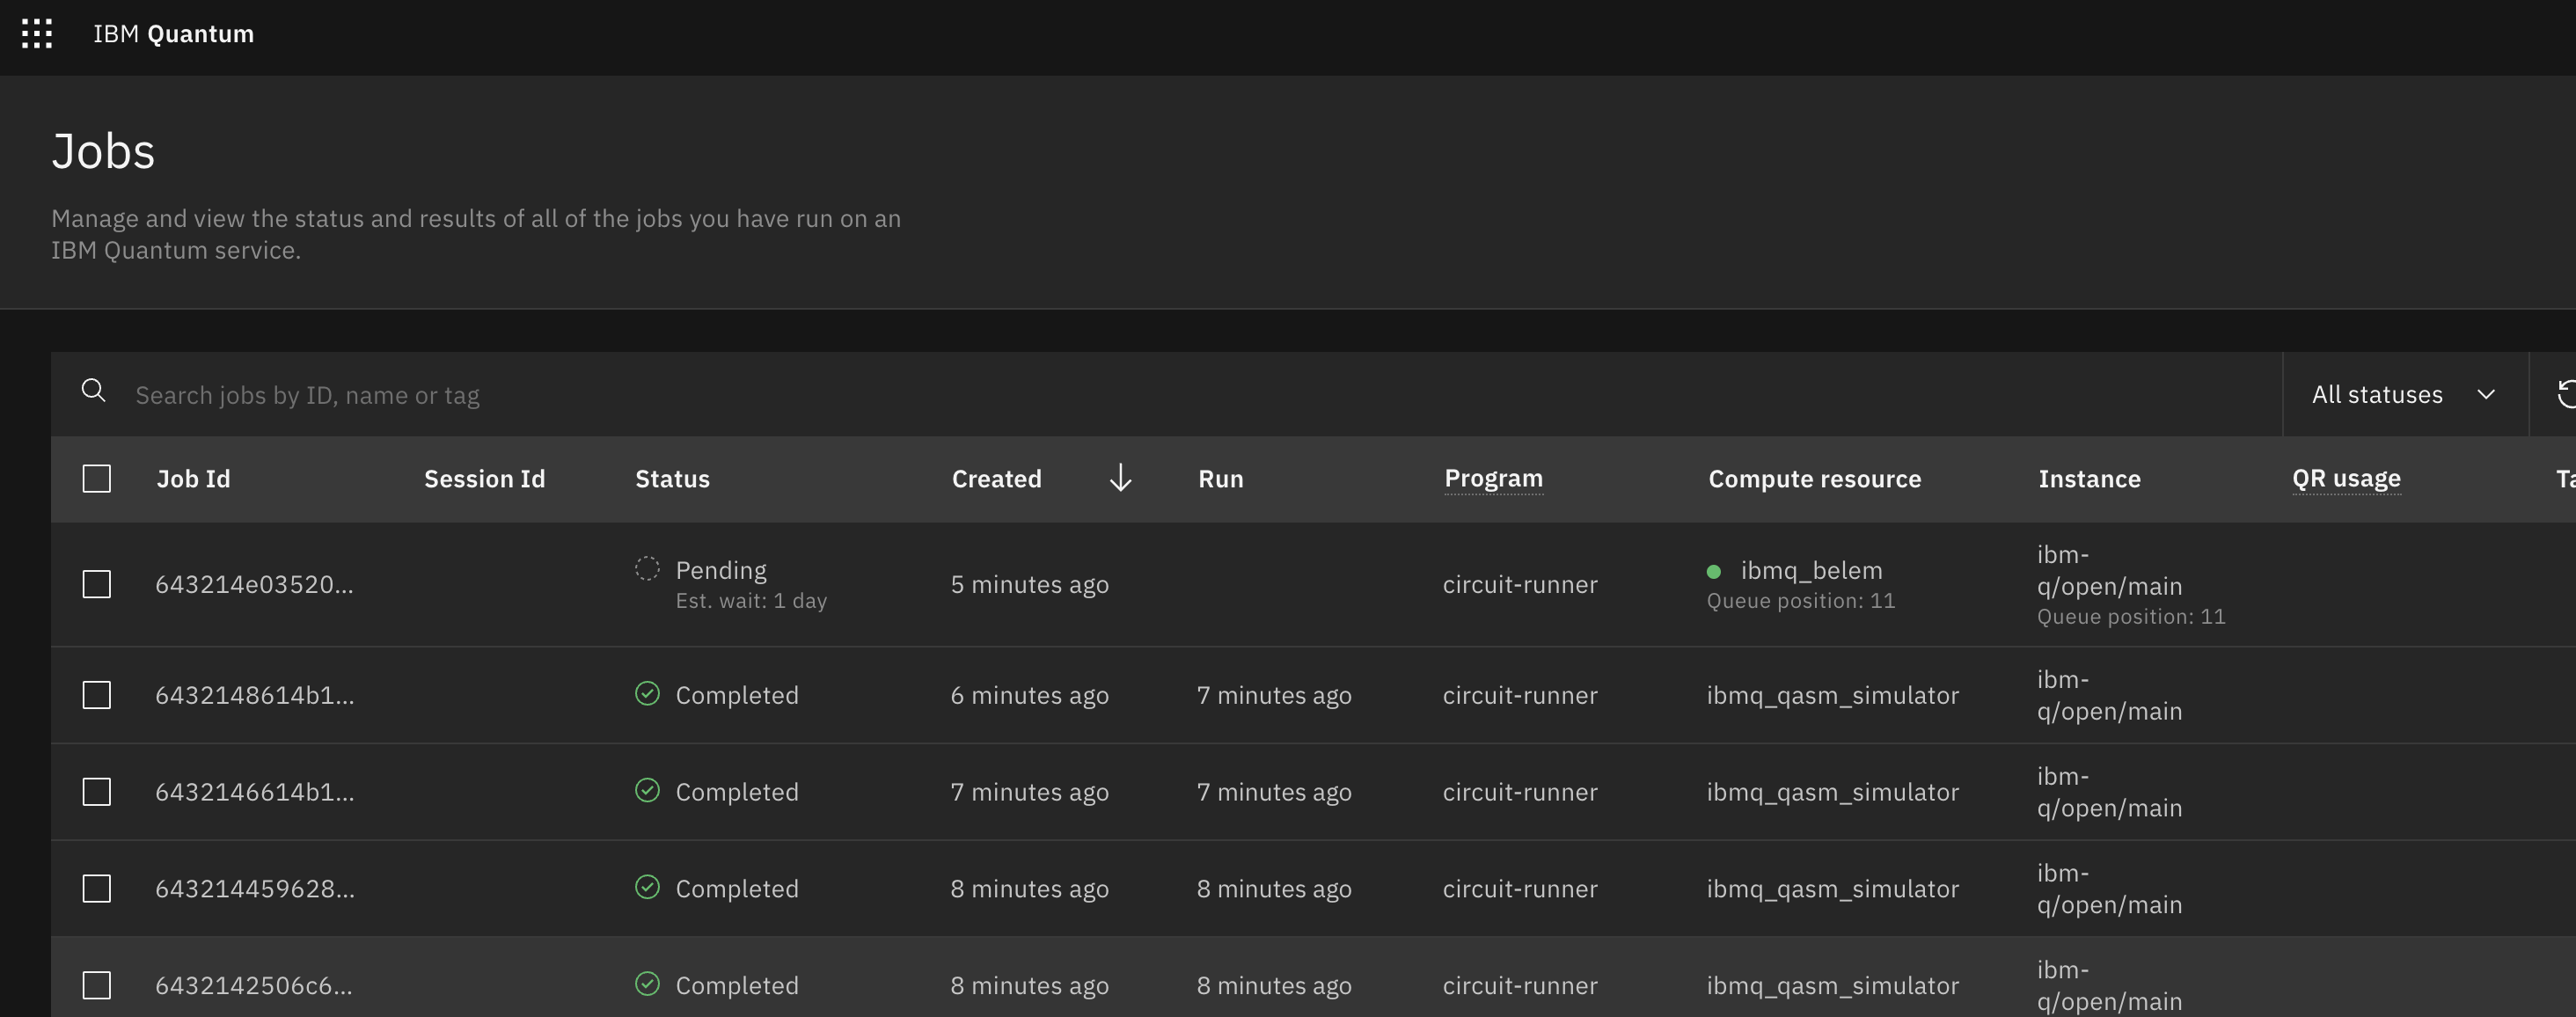
\includegraphics{figures/ibmq-wait-time.png}
    }
    \caption{IBMQ Wait Time}
    \label{fig:ibmq-wait-time}
\end{figure}

As a result, we fall back to the approach of simulating noise in the superconducting quantum processor. 

\subsection{Simulating Noise of the Real Quantum Processor}
We try to simulate the noise of the superconducting quantum processor using the Qisik Aer device \cite{aer}. Regarding the noisiness of the real device, the paper presents the energy relaxation time, dephasing time, probabilities of correct readout, and gate fidelities of each qubit in the real quantum processor, but it does not provide the gate time, which is required by Aer for simulating energy relaxation. We assume it is 130 nanoseconds, a typical time for single-qubit gates on superconducting quantum computers \cite{linke2017experimental}. Because of this missing information and the fact that we are unfamiliar with the underlying mechanics of physical quantum computers, the noise model we simulate could potentially deviate significantly from the actual quantum computer.

